\documentclass[10pt,a4paper]{report}
%\usepackage[utf8]{inputenc}
\usepackage[latin1]{inputenc}
\usepackage{amsmath}
\usepackage{amsfonts}
\usepackage{amssymb}
\usepackage{multicol, blindtext}
\usepackage{textcomp}
\usepackage{graphicx}
\usepackage{lipsum}

\title{Quantiza��o}

\begin{document}



%\title{Medi��o de Velocidade usando um Sensor de Luminosidade}

\author{Danilo Souza, Hugo Santos, Welton Ara�jo}
%Matr\'iculas: 10080000801, 10080000701, 10080000501}
%\thanks{Engenharia da Computa\c{c}\~ao, Universidade Federal do Par\'a, Bel\'em-PA, Brasil}
\maketitle

%Emails: \{dhcsouza, huggosan, weltonmaxx007\}@gmail.com\\

\section{Funcionamento}
O c�digo gera um sinal a partir de 2 sen�ides, uma com 1Hz  e outra com 2Hz de frequ�ncia. Em seguida, gera-se o sinal a uma taxa de amostragem de 500Hz com dura��o de 1 segundo. O objetivo principal � mostrar os efeitos do n�mero de n��veis de quantiza��o para efetuar a reconstru��o a partir do sinal amostrado capturado posteriormente nas taxas de amostragem 100Hz, 50Hz, 25Hz e 12.5Hz.

\section{Resultados}
Variando-se a taxa de amostragem descrescentemente, percebe-se que quanto maior ela era, melhor � a reconstru�ao de sinal amostrado. Por�m, diminuindo-se gradativamente, � poss��vel constatar a exist�ncia de um atraso onde o sinal reconstru�do. Al�m do atraso, o sinal capturado torna-se cada vez mais distorcido.

%\begin{multicols}{1}
\begin{figure}[h]
	\centering
	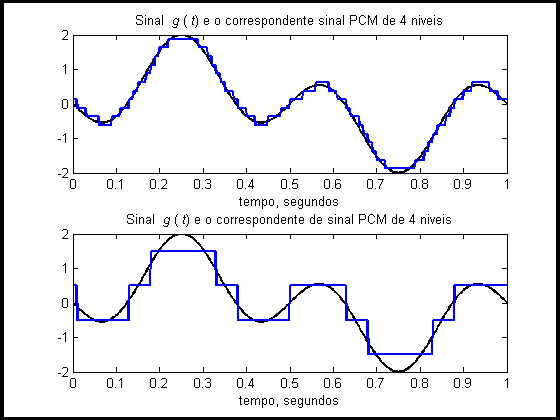
\includegraphics[scale=0.25]{./pictures/cap6CapTs001.png}
	%\caption{$ \alpha = 0.8$, N_t = 10, T_max = 2048}
	%\label{fig:semSolucao1}
\end{figure}
\begin{figure}[h]
	\centering
	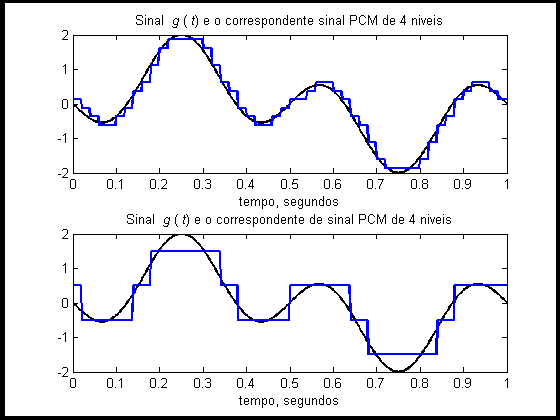
\includegraphics[scale=0.25]{./pictures/cap6CapTs002.png}
	%\caption{$ \alpha = 0.8$, N_t = 10, T_max = 2048}
	%\label{fig:semSolucao2}
\end{figure}
\begin{figure}[h]
	\centering
	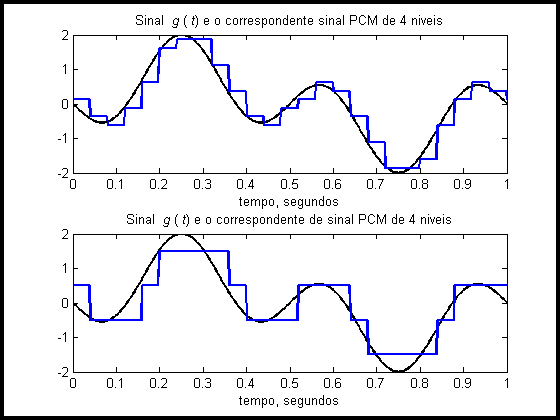
\includegraphics[scale=0.25]{./pictures/cap6CapTs004.png}
	%\caption{$ \alpha = 0.8$, N_t = 10, T_max = 2048}
	%\label{fig:semSolucao3}
	\end{figure}
\begin{figure}[h]
	\centering
	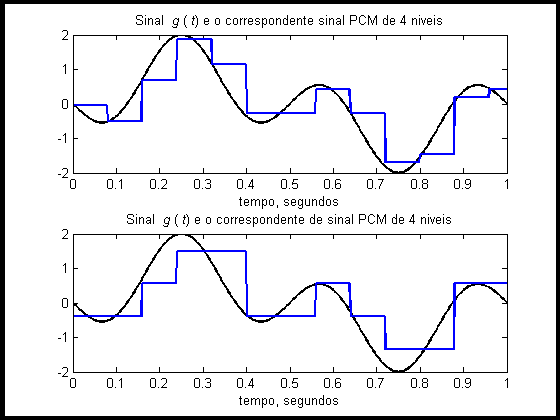
\includegraphics[scale=0.25]{./pictures/cap6CapTs008.png}
	%\caption{$ \alpha = 0.8$, N_t = 10, T_max = 2048}
	%\label{fig:semSolucao4}
\end{figure}
%\end{multicols}

A uma baixa taxa de amostragem, o quantizador de 16 bits mostrou uma grande perda de efici�ncia, pois os valores capturados por eles s�o visualmente pr�ximos do que se espera em taxas de amostragem mais altas, no entanto o grande espa�aamento entre as amostras faz com que a reconstru��o seja ineficiente.

Os efeitos do n�mero de n��veis do quantizador tiveram grande influ�ncia para que o sinal reconstru��do fosse mais parecido com o sinal original. Isto ocorre porque os valores do quantizador de 16 bits tem uma resposta mais pr�xima do valor amostrado. Portanto, uma precis�o mais alta, tamb�m tem grande influ�ncia para a reconstru�ao do sinal.

\end{document}